\chapter{Object Reconstruction and Selection}
\label{chap:object_reco}

\newpage

\section{Introduction}

%High-level overview
The CMS $H\rightarrow{\gamma\gamma}$ analysis works by searching for excess production in the distribution of diphoton invariant masses. A Higgs boson signal will manifest as a small bump on top of a continuous distribution due to background processes from Standard Model diphoton production.

The invariant mass of a diphoton system is calculated with the expression
\begin{equation}
    m_{\gamma\gamma} = \sqrt{2E_{\gamma_1}E_{\gamma_2}(1-\cos{\alpha})},
\end{equation}
where $E_{\gamma_1}$ and $E_{\gamma_2}$ are the energies of the leading energy photon and subleading energy photon respectively, and $\alpha$ is the opening angle between them. 
To determine the value of $\alpha$ we require the locations of the photons in the ECAL and the correct originating vertex. 
Good identification and measurement of photons and their verices are therefore crucial to the analysis, and the reconstruction of these will be described in detail in this chapter. 
Other objects such as jets and leptons provide extra information on signal events and allow for improved signal isolation. The reconstruction of these objects will also be described.

\section{ECAL Clusters and Particles}

ECAL clusters are used in many of the object of interest in this chapter and are especially important for photons. 
The clustering \cite{cmsEcalCalibration} begins with the identification of local energy maxima above a threshold value, these are referred to as seeds. 
After this topological clusters are grown from the seeds by gathering crystals which share at least one side with a seed, or crystals clustered with a seed, with energy above another threshold which is equal to $2\sigma$ of the ECAL electronic noise (up to 80\,MeV in the barrel and 300\,MeV in the endcaps).
Finally, these clusters are merged to form superclusters which allow for good energy containment, accounting for variation in the construction of the ECAL with $|\eta|$, and pileup robustness.



Physics objects are reconstructed with the CMS global event description known as particle flow (PF) \cite{ParticleFlow}.
PF uses information from all of the subdetectors to identify and reconstruct individual particles produced within CMS, and to achieve good energy resolution.
The information used as inputs are tracks from the tracker, tracks from the muon systems, and energy clusters from the ECAL and HCAL. Depending on which of these are present, PF will output `PF candidates' which correspond to different types of semi-stable particles 
\begin{itemize}[leftmargin=.5in,noitemsep]
    \item Photons: ECAL deposition is present with no associated track in tracker. The energy of photons is obtained from the ECAL. 
    \item Electrons: ECAL supercluster is present with associated track in tracker. Energy is determined with electron momentum at the primary vertex, the ECAL deposition, and the energy of associated Bremsstrahlung photons. 
    \item Muons: compatible tracks in tracker and muon system. Energy is determined from the curvature or the tracks. 
    \item Charged Hadrons: track in tracker, ECAL deposition and associated HCAL deposition. Energy is determined from the track curvature, and the matching ECAL/HCAL deposits corrected for effects from zero-suppression and for the response of the calorimeters to hadronic showers.
    \item Neutral Hadrons: measured with the corrected energies from the ECAL and HCAL. 
\end{itemize}
These PF candidates are then used to construct jets, and to determine missing transverse momentum $p_{T}^{miss}$.
This process is applied in the same way to data collected with the CMS detector and data from simulation.


\section{Samples}

\subsection{Trigger}
The analysis uses events selected with the two-step CMS triggering system (L1T and HLT). The objective of this system is to keep the event rate below an acceptable level due to limited bandwidth resources, whilst keeping signal efficiency a high as possible. Requirements at L1T are looser because it uses fast coarse measurement, HLT uses more stringent requirements to compensate for any inefficiencies from this. 

At L1T we require one or two energy deposits in the ECAL with energy thresholds that varied over the 2016 running period. For the single deposit, energy requirements are more stringent at 25\,GeV during low luminosity up to 40\,GeV at high-luminosity periods to keep the trigger rate to an acceptable level. For two deposits at high-luminosity 22\,GeV and 15\,GeV were required. 

At HLT events were selected with $E_{T}$ thresholds of 30\,GeV and 18\,GeV for the leading and subleading photon respectively. Furthermore, the selection has loose requirements on the shape of the electromagnetic showers, isolation variables, and the ratio of deposition in the ECAL compared to the HCAL. 

These selections have their efficiencies measured with the `tag-and-probe' technique \cite{TagAndProbe}. 
This uses the resonant production and decay to pairs of well-understood particles near their mass peak to ensure a pure and well-understood sample. 
In the $H\rightarrow{\gamma\gamma}$ analysis $Z\rightarrow{}e^{+}e^{-}$ is used as both electrons and photons are reconstructed with the ECAL clustering, so one can use di-electron decays as a proxy for diphotons. 
A strict ID requirement is placed on one of the decay products (the tag) and a looser requirement is placed on the other (the probe). 
The requirement on the probe should be loose enough that it does not affect the selection being measured. The selection efficiency may then be measured as the proportion of the probes which satisfy the selection.
%Ref for tag and probe from the PAS


\subsection{Data}
The data used in the analysis corresponds to the 35.9\,fb$^{-1}$ of proton-proton collision data recorded by the CMS experiment in the 2016 run period with a centre of mass energy of $s=\sqrt{13}$\,TeV and selected with the trigger requirements described above. 



\subsection{Simulation}

Simulated samples are used for a variety of tasks such as to train the ML models of the analysis, to optimise cuts and categorisations, producing signal models, and to perform validations. 

Signal events are simulated for a range of mass points from 120\,GeV to 130\,GeV using cross-sections and branching ratios recommended by the LHC cross-section working group. 
The signal events are generated at next-to-leading order in perturbative QCD with \texttt{MadGraph5_{}aMC@NLO}, with  parton showers and hadronization modelled with \texttt{pythia8}. The \texttt{pythia} tune parameter set \texttt{CUETP8M1} is used.

The background simulations are generated in different ways. For the main irreducible background from prompt diphotons \texttt{Sherpa} is used which includes Born processes with up to three jets as well as box diagram processes at leading order. 
For the $\gamma$-jet and jet-jet reducible backgrounds where jets are mistakenly reconstructed as photons we use \texttt{pythia8} with a filter applied to enhance the electromagnetic energy content of the jets. 
Finally, samples for validation $W\gamma$ and $Z\gamma$ are simulated with \texttt{Madgraph} and Drell-Yan (DY) is simulated with \texttt{Madgraph_{}aMC@NLO}


The CMS detector itself is simulated in detail with \texttt{GEANT4}. 
This includes the simulation of both in-time and out-of-time pileup. 
Simulated events are then weighted such that they reproduce the pileup distribution observed in data from CMS.






\section{Vertex Reconstruction}
If the selected vertex is within $1$\,cm of the correct vertex the contribution of spatial uncertainty to the mass resolution is negligible and is dominated by the energy resolution of the CMS ECAL. 
The ECAL gives a good determination of the photon location in $z$ and $\phi$, but it does not provide any pointing information: to determine $\alpha$ precisely we need to determine the correct vertex by other means.
When diphotons are produced in proton collisions there are also charged tracks present from jets or from the proton remnants which are associated to the same vertex. One can exploit this information to choose the correct vertex.  


The process begins by gathering the tracks in the central tracker and grouping them by their common points of origin. These are the candidate vertices. The next step will be to choose the vertex most compatible with the candidate diphoton under consideration.

\subsection{Vertex Selection}
Vertex selection is performed with a BDT classifier which takes a set of input features formed from the transverse momenta of tracks associated to the candidate vertex and the candidate diphoton. The features are
\begin{gather*}
    \sum_{i}|\vec{p}_{T}^{i}|^{2}. \\
    -\sum_{i}(\vec{p}_{T}^{i}\cdot\frac{\vec{p}_{T}^{\gamma\gamma}}{|\vec{p}_{T}^{\gamma\gamma}|}), \\
    (|\sum_{i}\vec{p}_{T}^{i}|-\vec{p}_{T}^{\gamma\gamma})/(|\sum_{i}\vec{p}_{T}^{i}|+\vec{p}_{T}^{\gamma\gamma}),
\end{gather*}
where $i$ enumerates the tracks of the candidate vertex. In the case of converted photons there are two additional features: the number of conversions and the pull $|z_{vtx} - z_{conv}|/\sigma_{z}$ where $z_{vtx}$ is the $z$ position from the vertex, $z_{conv}$ is the position estimated from the conversion tracks, and $\sigma_z$ is the uncertainty on $z_{conv}$.
The BDT is trained on vertices from simulated Higgs boson diphoton events with vertices which correspond to the true Higgs vertex considered the signal class and all others background. The selected vertex is then the candidate with the highest BDT score. 


\subsection{Vertex Probability}
Once a candidate vertex is selected, another BDT is used to score the probability that it is within $1$\,cm of the true vertex location.   
This is also trained on simulated Higgs diphoton events and is given the following input features,
\begin{itemize}[leftmargin=.5in,noitemsep]
    \item The number of vertices in the event.
    \item The three highest vertex ID scores.
    \item $p_{T}$ of the candidate diphoton.
    \item $\Delta{z}$ between the highest scoring vertex and the second highest.
    \item $\Delta{z}$ between the highest scoring vertex and the third highest.
    \item The number of converted photons.
\end{itemize}


\subsection{Performance}
Performance of the vertex selection BDT is validated with both simulated and real $Z\rightarrow{}\mu^{+}\mu^{-}$ events where the muon tracks have been removed and the event re-reconstructed to imitate a diphoton system. 
In the converted-photon case a similar procedure uses $\gamma + $jet events where the vertex is found using the tracks of the jet. 
The tracks of the jet are then removed and the event is re-reconstructed as a diphoton systems. Validation of unconverted photons is shown in Figure \ref{fig:object_reco:vertex_id_valid}. 
\begin{figure}[h!]
    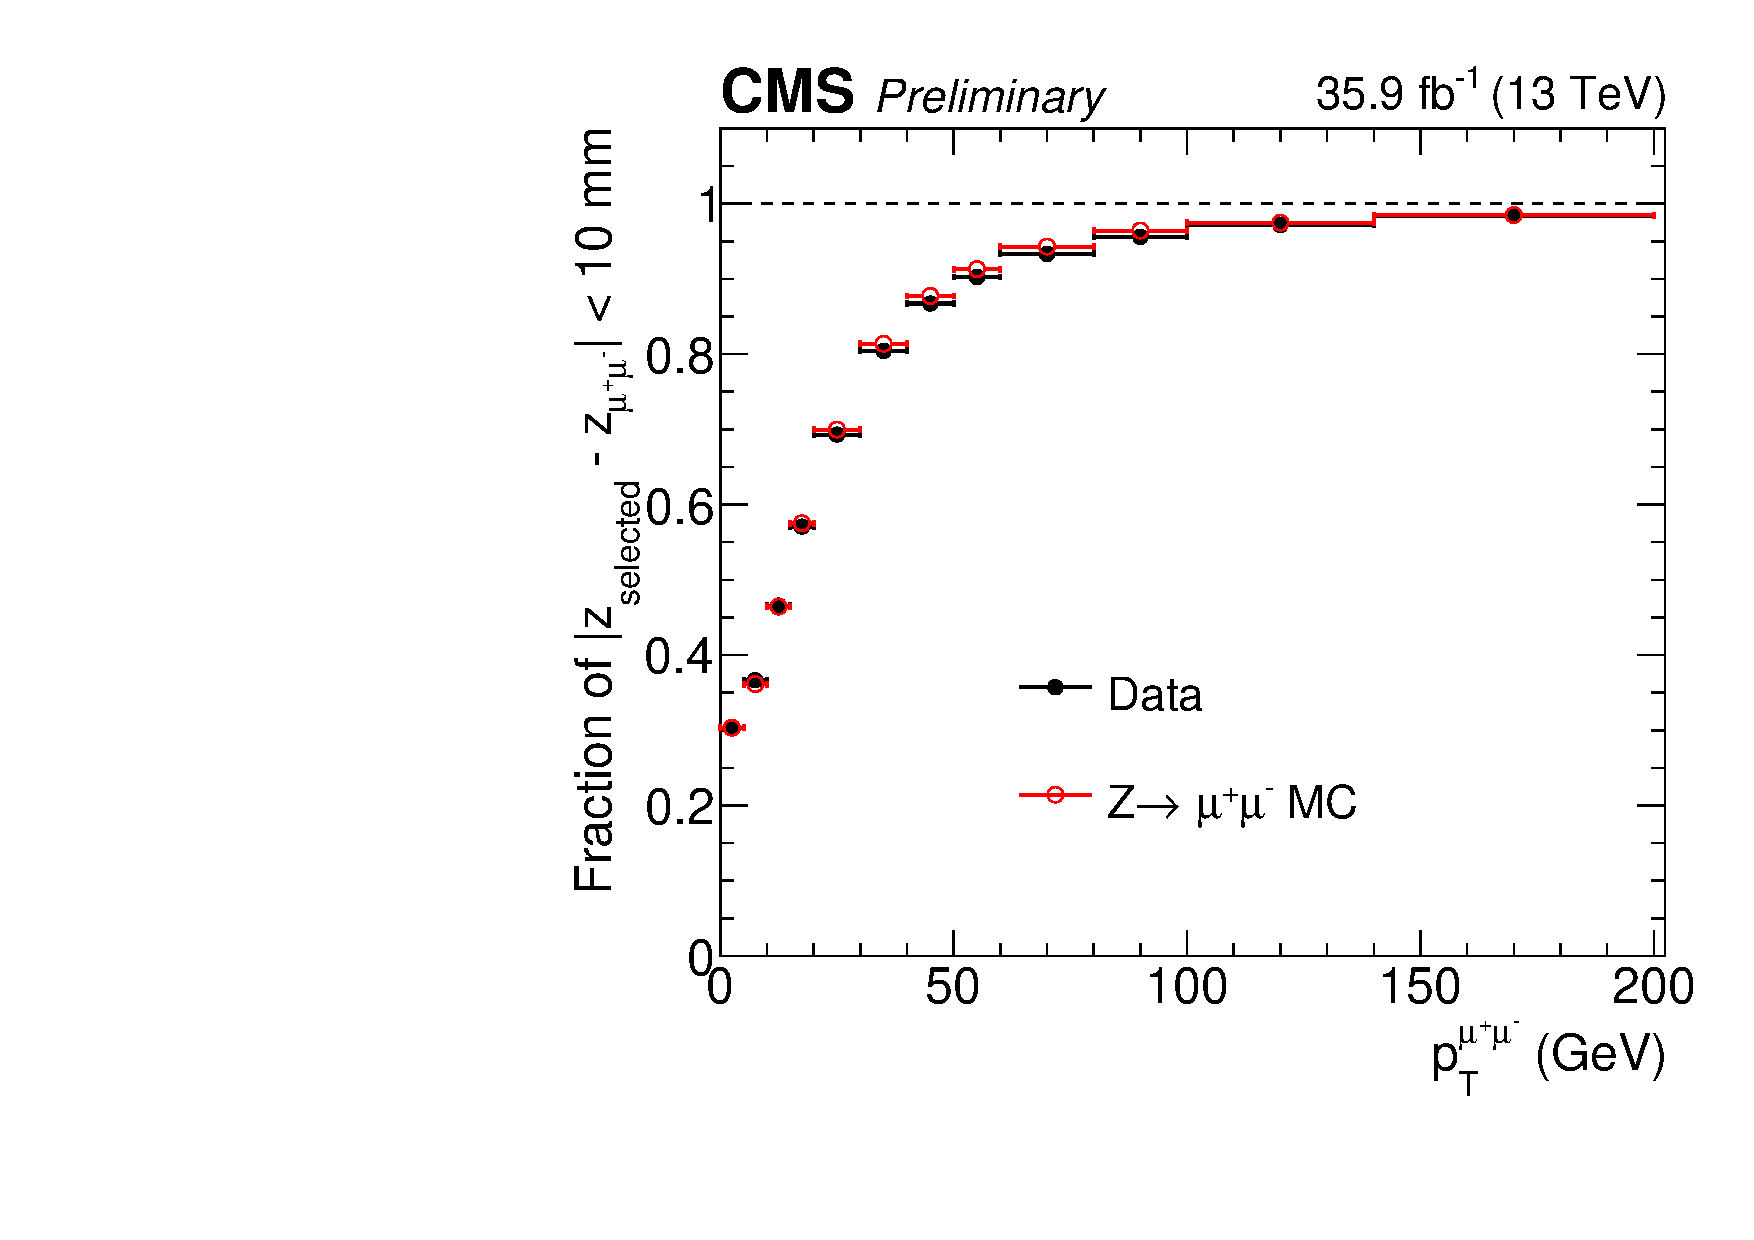
\includegraphics[width=0.45\textwidth]{figures/object_reco/CMS-PAS-HIG-16-040_Figure_003.pdf}
    \caption{Validation of vertex ID. Vertex ID efficiency in simulation and data for dimuon event reconstructed as diphotons.}
        \label{fig:object_reco:vertex_id_valid}
\end{figure}

The selection efficiency for selecting a vertex within $1$\,cm of the true position is evaluated using simulated Higgs diphoton decay events. This efficiency is shown for different bins of number of vertices in the event and the diphoton $p_{T}$ in Figure \ref{fig:object_reco:vertex_id_efficiency}. The efficiency over all events is approximately 81\%.
\begin{figure}[h!]
    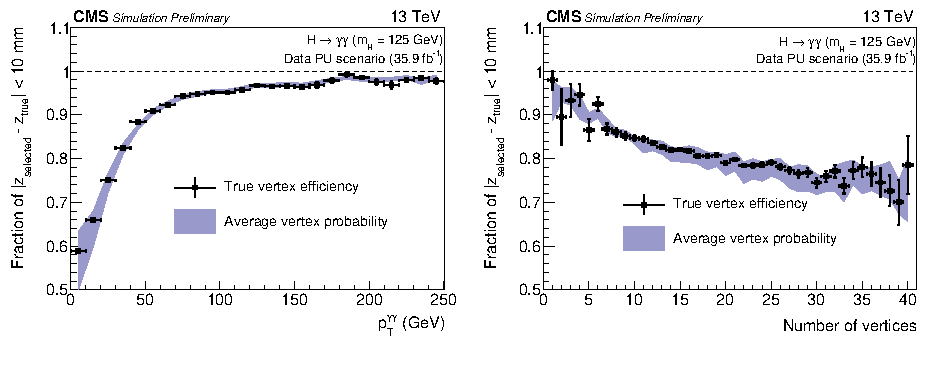
\includegraphics[width=0.95\textwidth]{figures/object_reco/CMS-PAS-HIG-16-040_Figure_004.pdf}
    \caption{Vertex ID efficiency as a function of diphoton $p_T$ (left) and number of event vertices (right).}
        \label{fig:object_reco:vertex_id_efficiency}
\end{figure}

Corrections are applied to account for discrepancies between data and simulation and a systematic uncertainty is assigned which is estimated by varying the ratio of data to simulation within their uncertainties. 

In simulated events the width of the distribution of beam spot longitudinal positions is a factor of $1.5$ wider than that measured in data. 
To compensate for this, simulated events with selected vertices more than $0.1$\,cm from the generator-level Higgs vertex are assigned a weighting that reproduces the width in data. 




\section{Photon Reconstruction}
Photons are reconstructed from calibrated ECAL superclusters which have had corrections calculated with a collection of techniques. One of these is a BDT regressor applied to account for detector effects. The resulting candidate photons are then put through a preselection aimed at rejecting non-prompt photons due to jet fragments, this also uses the output of a BDT classifier as a selection criterion.
All of these steps, including their validation, use a common collection of variables which will be detailed in the next subsection for later reference. 

\subsection{Common Variables}
The set of common variables can be divided into two main types: shower shape variables and isolation variables, plus some other miscellaneous variables. 
Shower shape variables describe properties of the electromagnetic showers within the ECAL which will allow us to infer information about the object. For example, whether a shower is from a pristine or a pair-converted photon.
The set of shower shape variables consists of the following:
\begin{itemize}[leftmargin=.5in,noitemsep]
    \item $E_{2\times{}2}/E_{5\times{}5}$: the ratio of energy in the $2\times{}2$ grid containing the most energetic crystal to the energy in the $5\times{}5$ grid around the SC seed crystal.
    \item $cov_{i\eta{i}\phi}$: the covariance of the crystal $\eta$ and $\phi$ locations within the $5\times{}5$ grid around the SC seed crystal. 
    \item $\sigma_{i\eta{}i\eta}$: pseudorapidity width of the shower in terms of crystals. 
    \item $R_{9}$: $E_{3\times{}3}/E_{SC}$, the ratio of the energy in the $3\times{}3$ grid around the SC seed crystal to the energy of the SC.
    \item $\sigma_{\eta}$: the logarithmic energy-weighted standard deviation of crystal $\eta$ in a SC.
    \item $\sigma_{\phi}$: the logarithmic energy-weighted standard deviation of crystal $\phi$ in a SC.
    \item $\sigma_{rr}$: the standard deviation of the shower width in the $x-y$ plane as measured by the preshower (only for photons measured in the endcaps).
\end{itemize}


Isolation variables measure how well-separated an object, in this case a photon, is from other objects in the event such as electrons or charged hadrons which could imitate the true signal. The set of isolation variables consists of the following
\begin{itemize}[leftmargin=.5in,noitemsep]
    \item $\mathcal{I}_{\gamma}$: photon isolation, the sum of the transverse energy of the particles identified as photons in a cone of $R=0.3$ around the candidate photon.
    \item $\mathcal{I}^{V}_{\mathrm{CH}}$: charged hadron isolation, the sum of transverse momenta of charged particles in a $R=0.3$ cone around the candidate photon associated with vertex $V$. 
    \item $\mathcal{I}_{\mathrm{T}}$: track isolation, the sum of transverse momenta of tracks in a hollow cone between $R=0.3$ and $R=0.04$ around the candidate photon.
    \item $H/E$: the ratio of energy measured in the HCAL to the energy measured in the ECAL in a cone of $R=0.15$ around the candidate photon.
\end{itemize}

Finally there are other miscellaneous variables used throughout the selection for different purposes,
\begin{itemize}[leftmargin=.5in,noitemsep]
    \item Electron veto: true or false if there is a track associated with the candidate SC.
    \item $\rho$: the event median energy density per unit area.
    \item $\eta_{SC}$: the pseudorapidity of the candidate SC.
    \item $E_{SC}^{RAW}$: the uncorrected energy of the candidate SC.
\end{itemize}



\subsection{Photon Energy Corrections}

The photon energy has a set of corrections applied depending on whether the photon is from simulation or data: individual photon energy correction, an overall energy scale correction in data, and a smearing of the simulated data to match its distribution to data. 

\subsubsection{Photon Energy Correction}
The photon energy correction is computed with a regressor BDT whose target is the ratio of true energy to the raw measured energy of the associated supercluster. It also computes the median uncertainty of the energy. 
The inputs to the BDT are a collection of shower shape variables, position variables, information from the preshower subdetector, and pileup-sensitive event-level variables.
The BDT is then trained on simulated photons with two separately trained BDTs in the barrel and endcap regions. 


\subsubsection{Energy Scale}
Once we have the corrected energies, the overall energy scale needs to be corrected to account for detector effects. 
During operation the CMS ECAL receives large doses of radiation that can degrade its performance over time. 
This will lead to drifts and jumps in the detector response as conditions change, and as a result the measured energy will also drift and jump. 
Scale factors to account for this effect in data are calculated using the $Z\rightarrow{}e^{+}e^{-}$ decay as a standard candle where the electrons are reconstructed as photons. 
Using comparison to simulation, and the well-known value of the $Z$ boson mass, scales are derived for different times and detector locations to bring the measured value of real $Z$ bosons back to the true value. 


\subsubsection{Resolution Smearing}
Simulation also needs to be corrected by comparison to data to make it more realistic. The photon energy resolution in simulated events has a Gaussian smearing added to it which is derived from comparing the width of the $Z\rightarrow{}e^{+}e^{-}$ mass distribution in different categories depending on $|\eta|$-location within the detector (two in the barrel either side of $|\eta|=1$ and two in the endcaps either side of $|\eta|=2$), and the $R_{9}$ variable which measures photon quality (above or below $R_{9}=0.94$).
The mass peak in two of these bins is shown in Figure \ref{fig:object_reco:invariant_mass_validation}.
\begin{figure}[h!]
    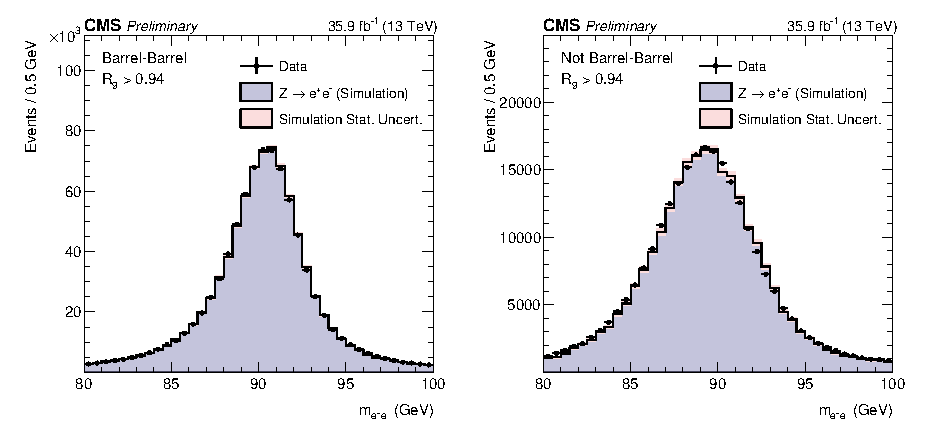
\includegraphics[width=0.95\textwidth]{figures/object_reco/CMS-PAS-HIG-16-040_Figure_001.pdf}
    \caption{A comparison between data and simulation of dielectron invariant mass}
        \label{fig:object_reco:invariant_mass_validation}
\end{figure}

\subsection{Photon Preselection}
%intro
Before a photon can enter the analysis it must pass a set of selection criteria, the photon preselection, which are slightly more stringent than the trigger and vary by location. First photons are grouped into candidate diphotons by considering all possible pairs in the event, then the criteria are applied (with the exception of $p_{T}$ cuts) on a per-photon basis.
The criteria are:
%List of requirements
\begin{itemize}[leftmargin=.5in,noitemsep]
    \item Electron veto: rejection if there is a track associated to the supercluster.
    \item Photon $p_{T}$s: $p_{T}^{\gamma_1} > 30$\,GeV and $p_{T}^{\gamma_2} > 20$\,GeV
    \item $R_{9}$: is not used to reject events outright, but determines which other selections are applied. If $R_{9} < 0.85$ in the barrel or $R_{9} < 0.9$ in the endcaps additional requirements are imposed. 
    \item Energy-weighted $\eta$ width: $\sigma_{\eta\eta} < 0.015$ in the barrel and $\sigma_{\eta\eta} < 0.015$ in the endcaps
    \item HCAL/ECAL deposition: $H/E < 0.08$ in all regions.
    \item Photon isolation: $\mathcal{I}_{\gamma} < 4.0$ in all regions. 
    \item Track isolation: $\mathcal{I}_{T} < 6.0$ in all regions.
    \item Charged hadron isolation: $\mathcal{I}_{CH} < 20$\,GeV.
    \item Photon ID: score from a BDT classifier that discriminates between prompt photons and jet fragments.
\end{itemize}
Both photons must also satisfy either of two additional requirements:
\begin{itemize}[leftmargin=.5in,noitemsep]
    \item $R_{9} > 0.8$ and $\mathcal{I}_{CH} < 20$\,GeV
    \item $\mathcal{I}_{CH}/p_{T}^{\gamma} < 0.3$
\end{itemize}

%Schema table of thesholds
The efficiency of these criteria are measured using $Z\rightarrow{}e^{+}e^{-}$ and the tag-and-probe method, 
with the exception of the electron veto which uses $Z\rightarrow{}\mu^{+}\mu^{-}\gamma$. The preselection efficiencies are summarised in Table \ref{tab:object_reco:presel_eff}
%Table of efficiencies
\begin{table}[h!]
    \begin{tabular}{ l | c | c | c }
        Preselection Category& $\epsilon_{\mathrm{data}} (\%)$ & $\epsilon_{\mathrm{sim}} (\%)$ & $\epsilon_{\mathrm{data}}/\epsilon_{\mathrm{sim}}$ \\
        \hline
        Barrel, $R_{9}>0.85$ & $94.2\pm0.9$ & $94.7\pm0.9$ & $0.995\pm0.001$ \\
        Barrel, $R_{9}<0.85$ & $82.5\pm0.7$ & $82.5\pm0.7$ & $1.000\pm0.003$ \\ 
        \hline
        Endcap, $R_{9}>0.85$ & $90.1\pm0.2$ & $91.3\pm0.1$ & $0.987\pm0.005$ \\ 
        Endcap, $R_{9}<0.85$ & $49.7\pm1.4$ & $53.8\pm1.5$ & $0.923\pm0.010$ \\ 
\end{tabular}
    \caption{Preselection efficiencies}
    \label{tab:object_reco:presel_eff}
\end{table}





\subsection{Photon Identification}
%Intro
The photon identification BDT is a classifier whose task is to discriminate between real prompt photons and photon-like jet fragments which satisfy the preselection criteria. 
The BDT is trained using simulated $\gamma + $jet events where the reconstructed photons are matched to a generator-level particle, if there is no match it is considered to be in the non-prompt class.
To avoid the BDT introducing a dependence on on photon kinematics the signal photons are re-weighted such that their distribution in $p_{T}$ and $\eta$ is flat. 
The classifier receives the following input features:
%variables
\begin{itemize}[leftmargin=.5in,noitemsep]
    \item Shower shape features: $\sigma_{i\eta{}i\eta}$, $cov_{i\eta{}i\phi}$, $E_{2\times{}2}/E_{5\times{}5}$, $R_{9}$, $\sigma_{\eta}$, $\sigma_{\phi}$, and $\sigma_{rr}$
    \item Isolation features: $\mathcal{I}_{\gamma}$, $\mathcal{I}_{CH}^{SV}$, and $\mathcal{I}_{CH}^{WV}$, where $SV$ and $WV$ refer to the selected vertex and worst vertex in terms of the vertex probability BDT respectively. 
    \item Other features: $\rho$, $\eta_{SC}$, $E_{SC}^{RAW}$, and $E_{ES}/E_{SC}^{RAW}$ where $E_{ES}$ is the energy measured by the ECAL preshower (endcaps only).
\end{itemize}

%validation 
The performance of this classifier is shown in Figure \ref{fig:object_reco:photon_id_bdt}. 
The systematic uncertainty on the BDT output is shown by the shaded region of the right hand plot. This is estimated so that it covers the largest disagreement between data and simulation of $Z\rightarrow{e^{+}e^{-}}$ reconstructed as photons in the endcap regions where agreement is worst.
\begin{figure}[h!]
    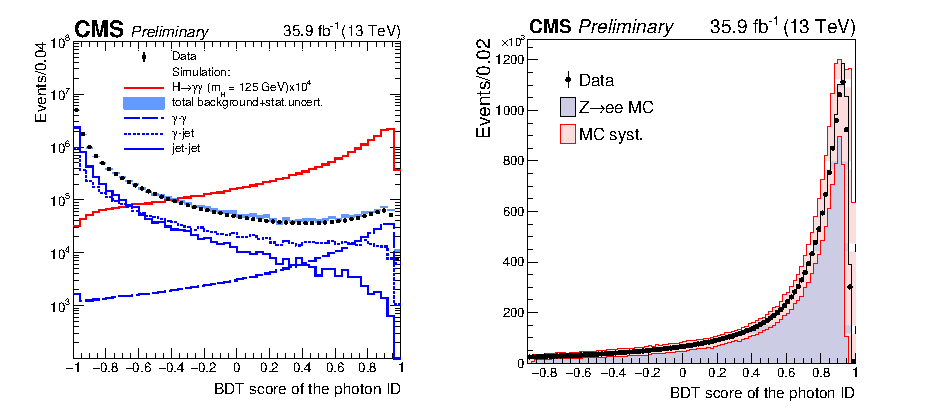
\includegraphics[width=0.95\textwidth]{figures/object_reco/CMS-PAS-HIG-16-040_Figure_002.pdf}
    \caption{Photon ID BDT performance and validation. (Left) Photon ID BDT output score of the lower-scoring photon of each diphoton passing the photon preselection. Signal photons from simulated Higgs events are shown in red and simulated background events are shown in blue, data is shown by the back dots. (Right) validation on $Z\rightarrow{e^{+}e^{-}}$ events.}
        \label{fig:object_reco:photon_id_bdt}
\end{figure}

A loose selection this BDT score is imposed as part of the photon preselection: $\hat{y} > -0.9$ where $\hat{y}$ is the output value. This selection keeps $99\%$ of the signal and removes a large portion of the background. This score is also used in later steps as a measure of photon quality: whether the photon is well-isolated and unconverted, or not. 


\section{Other Objects}

\subsection{Leptons}
Leptons are used for validation purposes throughout the analysis, and also event categorisation where there are leptons in the final state such as production with the ttH or VH modes. 
\subsubsection{Electrons}
Electrons are reconstructed in a similar way to photons, but with the extra requirement of an associated track. This association can be achieved in two ways depending on the properties of the candidate:
\begin{itemize}
    \item ECAL-based: starting with an energetic and well-isolated ECAL SC, match the track that is closest to the energy-weighted position of the SC and also within a window of $\Delta\eta=0.02$, $\Delta\phi=0.15$ of it.
    \item Tracker-based: starting with candidate tracks, associate them to a geometrically compatible SC. This is used for low $p_{T}$ electrons ($p_{T} < 10$\,GeV).
\end{itemize}
Candidates from both methods are combined to produce the set of PF candidate electrons of the event. 
There are also corrections applied to the tracks to correct for bremsstrahlung effects, and an energy correction from a BDT regressor analogous to the photon reconstruction. 

\subsubsection{Muons}
Hits in the muon system are formed into track segments and these are assembled via a clustering algorithm into muon system tracks called standalone muons. 
These are then associated with tracks from the inner tracker to produce global muons. A third approach is also used where inner tracks with $p_{T}<0.5$\,GeV and total $p < 2.5$\,GeV are extrapolated into the muon system. If a compatible muon segment is found this makes a `tracker muon'. Global muons and tracker muons that share the same inner track are merged into a single candidate. 
Standalone muons have worse momentum resolution and are more influenced by cosmic rays.

\subsection{Jets}
Jets are composite objects reconstructed from PF candidates using the anti-$k_T$ algorithm \cite{AntiKt} with $R=0.4$. 
The dedicated calibration for each PF candidate type, as well as 90\% of the jet energy being in the form of photons and charged hadrons allows for high-resolution measurement with the inner tracker and ECAL. The remaining 10\% consists of neutral hadrons which are measured at lower energy resolution in the HCAL \cite{JetPerformance}. 
The tracks also allow for the identification and rejection of particles originating from pileup vertices. Pileup gives extra energy to signal jets, and the soft pileup jets of these interactions can also be clustered into so-called fake jets of relatively large $p_{T}$ when they overlap. This latter effect rises quadratically with the number of pileup interactions. 

The jet objects receive corrections to their energy which relate the energy of the reconstructed jets to the energy at particle-level. A factorised approach is used \cite{JetPerformance}:
\begin{itemize}[leftmargin=.5in,noitemsep]
    \item First: subtracts $p_{T}^{offset}$ due to pileup influence. This is an average correction derived from the global per-event density $\rho$
    \item Second: corrects $p_{T}$ and $\eta$ dependence of the average jet detector response due to non-linearities in the calorimetry, differences in construction as a function of $\eta$, and $p_{T}$ thresholds.
    \item Jet energy scale: corrections for average residual discrepancies between data and simulation
\end{itemize}

In this analysis a collection of pileup mitigation techniques are employed. First, charged hadrons from vertices other than the chosen vertex are ignored within the tracker acceptance where this information is available. Outside the tracker a selection criterion is placed on the width of the jet expressed as
\begin{equation}
    \sigma_{RMS} = \frac{\sum_{i}p_{T}^{i^2}\Delta{R}^{i}}{\sum_{j}p_{T}^{j^2}}
\end{equation}
where $\Delta{R}^{i}$ is the distance between the constituent and the jet axis. The requirement is that $\sigma_{RMS} > 0.03$. 
Finally another technique uses a BDT classifier that takes a collection of jet shape variables and produces a score for each jet. A collection of selections on this score are then applied for bins in $p_{T}$ and $\eta$ (Table \ref{tab:object_reco:tight_pujid}).
Finally, in addition to the above, all jets are required to be within $|\eta| < 4.7$.

\begin{table}[h!]
    \begin{tabular}{ l || c | c | c | c }
         & $|\eta| < 2.5$ & $2.5 \leq |\eta| < 2.75$ & $2.75 \leq |\eta| < 3.0$ & $3.0 \leq |\eta| < 5.0$ \\
        \hline
        \hline
        $20 < p_{T} \leq 30$  & $0.69$ & $-0.35$ & $-0.26$ & $-0.21$ \\
        $30 < p_{T} \leq 50$  & $0.86$ & $-0.1$  & $-0.05$ & $-0.01$ \\
        $50 < p_{T} \leq 100$ & $0.95$ & $0.28$  & $0.31$  & $0.28$  \\
\end{tabular}
    \caption{Pileup jet ID cuts of the tight working point}
    \label{tab:object_reco:tight_pujid}
\end{table}





